\section{Motivation}
\label{sec:motivation}

\subsection{Abstractions of 1Pipe}
\label{subsec:abstration}

\RED{Explain the magic sauce of \sys{}.}

\sys{} provides a \emph{causally and totally ordered} communication abstraction in a distributed system with multiple hosts, where each host has multiple processes. Each host maintains a monotonically increasing timestamp, which represents the wall clock and is synchronized among all hosts. A message consists of one or more packets. When a process sends a group of messages (\emph{i.e.}, a \emph{scattering}) to different destinations, all packets of the messages are labeled with a same timestamp of the sender host. The total order property is: \emph{each process receives messages from different hosts in non-decreasing timestamp order}. The causality property is: \emph{when a process receives a message with timestamp T, timestamp of the host must be higher than T}.

\begin{table}[htbp]
\centering
\begin{tabular}{l}
	\hline
	TS = onepipe\_unreliable\_send(vec[<dst, msg>]) \\
	\hline
	TS, src, msg = onepipe\_unreliable\_recv() \\
	\hline
	onepipe\_send\_fail\_callback(func(TS, dst, msg)) \\
	\hline
	\hline
	TS = onepipe\_reliable\_send(vec[<dst, msg>]) \\
	\hline
	TS, src, msg = onepipe\_reliable\_recv() \\
	\hline
	onepipe\_proc\_fail\_callback(func(proc, TS)) \\
	\hline
	\hline
	TS = onepipe\_get\_timestamp() \\
	\hline
	onepipe\_init() \\
	\hline
	onepipe\_exit() \\
	\hline
\end{tabular}
\caption{Programming API of \sys{}. Vec[<dst, msg>] indicates a scattering of messages that have a same timestamp.}
\label{tab:abstraction}
\end{table}

As Table~\ref{tab:abstraction} shows, \sys{} provides two services with different reliability guarantees: first, \textit{onepipe\_unreliable\_recv} is a \emph{best effort} service where packet loss is possible, and \sys{} guarantees that delivered messages satisfy causal and total order properties. %\textit{onepipe\_unreliable\_recv} returns all messages with a same timestamp.
Modern data centers with advanced congestion control~\cite{kumar2020swift,hu2020aeolus,perry2015fastpass,gao2015phost} have very low packet loss rates, because congestion loss has been almost eliminated, and packet losses are mainly due to packet corruption. Packet corruption rate should be below $10^{-8}$ according to IEEE 802.3 standard, and links with corruption rate higher than $10^{-6}$ are considered to be faulty~\cite{zhuo2017understanding}.
%There have been works~\cite{ports2015designing,eris} that leverage low packet loss rate in data centers.
So, the application can assume that best effort \sys{} is almost reliable, but should guard against the failure cases.
Best effort \sys{} does not retransmit packets.
The application should use \textit{onepipe\_send\_fail\_callback} to detect lost packets and possible remote host failure.

Second, \textit{onepipe\_reliable\_recv} is a \emph{reliable} service which in addition to ordering, guarantees reliability: \emph{a message is guaranteed to be delivered if both sender and receiver processes do not fail}.
The reliable service retransmits packets in the case of packet loss.
In this paper, we only consider crash failures.
When a process or network fails, message delivery stalls.
\sys{} removes in-flight messages from or to the failed process.
If a message cannot be delivered, the send failure callback is invoked.
In addition, each process may register a callback function via \textit{onepipe\_proc\_fail\_callback} to get notified of failed processes.
Message delivery is resumed after all correct processes finish their callback functions.

Reliable \sys{} also provides \emph{restricted failure atomicity}, which means all-or-nothing delivery of \emph{a batch of messages} with the exception that if a receiver fails \emph{permanently} or network partitions after the decision to deliver is made, the receiver can never deliver it.
Specifically, atomicity is guaranteed on sender failure.
If receivers recover from failure, they deliver or discard messages consistently with correct receivers.
In fact, full failure atomicity is impossible in a non-replicated fail-stop model, because a receiver or its network link may fail permanently before delivering $T$ almost simultaneously with another receiver delivering $T$~\cite{fischer1985impossibility}.
Applications may solve permanent failures with replication and traditional consensus algorithms~\cite{lamport1998part,raft}.
%As we will show in Sec.~\ref{sec:reliable}, compared to best effort \sys{}, reliable \sys{} adds one RTT to message delivery.

\iffalse
\textcolor{red}{Outline:\\
1. What is message scattering?\\
2. Ordering anomalies. List several examples.\\
3. what is Total-Order message scattering? and why it is important. Recall the above examples / applications.\\
4. Challenges to provide total-order message scattering.\\
}
\fi

\subsection{Use Cases of 1Pipe}
\label{subsec:application}

\subsubsection{Total Ordering of Communication Events}
\label{subsec:order-hazards}

\begin{figure}[t]
\centering
	\subfloat[Write after write.\label{fig:ordering-waw}]
	{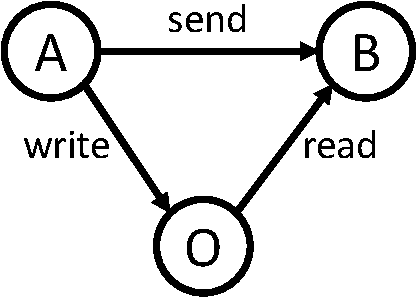
\includegraphics[width=.17\textwidth,page=1]{images/ordering-cropped.pdf}}
    \hspace{0.02\textwidth}
    \subfloat[Independent read, independent write.\label{fig:ordering-iriw}]
	{\includegraphics[width=.18\textwidth,page=2]{images/ordering-cropped.pdf}}
    %\hspace{0.01\textwidth}
	%\subfloat[Independent multi-write.\label{fig:ordering-imw}]
	%{\includegraphics[width=.11\textwidth,page=3]{images/ordering-cropped.pdf}}
	\caption{Ordering hazards in a distributed system.}
	\label{fig:ordering}
\end{figure}


%Message scattering is a common communication pattern in distributed systems, where one end-host sender sends a group of messages to one or more end-host receivers.
%First, packet losses can occur due to congestion, packet corruption and network switch or link failure.
%Packet losses and host failures may violate atomicity of message scattering.
With different delays of network paths, several categories of ordering hazards~\cite{gharachorloo1990memory,sewell2010x86} may take place (Figure~\ref{fig:ordering}).

\parab{Write after write (WAW).}
Host $A$ writes data to another host $O$, then sends a notification to host $B$. Send can be considered as a write operation.
When $B$ receives the notification, it issues a read command to $O$, but may not get the data due to message delays.

\parab{Independent read, independent write (IRIW).}
Host $A$ first writes to data $O_1$ and then writes to metadata $O_2$. Concurrently, host $B$ reads metadata $O_2$ and then reads data $O_2$.
It is possible that $B$ reads the metadata from $A$ but the data is not updated yet.

%IRIW hazard is common in shared data structures, where metadata and data needs to be accessed together atomically. %Note that messages to $O_1$ and $O_2$ may be different, so it is a \textit{scattering} instead of multicast.

%\parab{Independent multi-write (IMW)}.
%Host $A$ scatters writes to both $O_1$ and $O_2$. Concurrently, $B$ also scatters writes. The ordering of $A$'s and $B$'s writes at $O_1$ and $O_2$ may be different, causing inconsistency. % For example, if $O_1$ and $O_2$ are two replicas, IMW hazard would lead to inconsistent histories between replicas. %In replication, a log is sent to replicas as multicast. However, other scenarios still need the scattering semantics. For instance, if $A$ and $B$ are web servers, $O_1$ collects access log and $O_2$ collects error log, then logs for each HTTP request are scattered to different hosts.
%$S_1$ and $S_2$ are two web servers, generating an access log to $A$ and an error log to $E$ for each HTTP request.
%The interleaving order of requests from $S_1$ and $S_2$ may be different \REDBLU{between}{at} $A$ and $E$.

Ordering hazards affect system performance. To avoid the WAW hazard, $A$ needs to wait for the first write operation to complete (an RTT to $O$, called a \emph{fence}) before sending to $B$, thus increasing latency. To avoid the IRIW hazard, $A$ needs to wait for write $O_1$ to complete before initiating write $O_2$, and $B$ needs to wait for read $O_2$ to complete before initiating read $O_1$. The fence latency will be exaggerated when multiple remote objects need to be accessed in order.

%In today's distributed systems, to avoid WAW hazards, $A$~\textcolor{red}{$A$ is not defined here. gefei:'A is defined in Figure~\ref{fig:causality_traditional}'} needs to wait for the first write operation to complete (an RTT to the shared storage) until issuing the next operation, therefore increases latency and limits concurrency.~\textcolor{red}{thus increasing latency and degrading the throughput?}
%To avoid IMW and IRIW hazards, application needs locks or explicit coordination via logical timestamps~\cite{lamport1978time}.

\sys{} can remove both WAW and IRIW hazards due to causality and total ordering.
In WAW hazard, by monotonicity of host timestamp, $A \rightarrow O$ is ordered before $A \rightarrow B$. By causality, $A \rightarrow B$ is ordered before $B \rightarrow O$.
Consequently, $A \rightarrow O$ is before $B \rightarrow O$.
Therefore, the write operation is delivered before the read operation, thus avoiding WAW hazard.
Because the fence between $A \rightarrow O$ and $A \rightarrow B$ is removed, the end-to-end latency is reduced from 2.5 RTTs to 1.5 RTTs.

%\RED{causal order: avoid failure cases, e.g., A fail to write to B, A send to C will also fail. (reliable \sys{})}

%\RED{Why not let the application provide dependency among messages? Can remove false dependency in \sys{}. isis labeling psync, but cannot improve performance by much (cite ken birman response to understanding the limits)}

If an application needs to process a lot of WAW communication tasks \emph{in sequence}, the power of \sys{} is amplified. Using the traditional method, the application needs 1 RTT of idle waiting during each WAW task, so, the throughput is bounded by 1/RTT. Using \sys{}, the application can send messages in pipeline, so, the throughput is only limited by computation speed and network bandwidth.

The argument above neglects possible packet loss.
In best effort \sys{}, there is a small possibility that message $A \rightarrow O$ is lost in flight, so $B$ still needs to check the version of $O$ after reading. If it does not match $A$, then $B$ needs to wait for $A$ to retransmit $O$ and re-notify $B$.
$A$ registers send failure callback and performs rollback recovery when $A$ is notified of a send failure.
If we use reliable \sys{}, $O$ does not need to maintain a version, but it adds an RTT to each message delivery, so, the end-to-end latency increases from 2.5 to 3.5 RTTs. However, $A$ can still send messages in pipeline, and have much higher throughput than the traditional way.
In addition, reliable \sys can preserve causality in failure cases~\cite{birman1994response}: if $A$ fails to write to $O$, message $A \rightarrow B$ will not be delivered, similar to Isis~\cite{birman1984overview}.

Similarly, \sys{} removes IRIW hazard and improves minimum end-to-end latency from 3 RTTs to 1 RTT because two fences are removed. The minimum latency is achieved when $A$ and $B$ initiate read and write simultaneously.

The ability to totally order communication events is the root power of removing ordering hazards.
This power is also a perfect match with \textit{total store ordering} (TSO) memory model~\cite{sewell2010x86} in a distributed shared memory (DSM) system. In TSO, each processor observes a consistent ordering of writes from all other cores. In other words, processors must not observe WAW and IRIW hazards.
Compared to weaker memory models, TSO reduces synchronization in concurrent programming~\cite{morrison2013fast,tassarotti2015verifying}, thereby simplifying programming and reducing fence overheads.

\subsubsection{Replication}

%The global timestamp not only gives ordering, but also gives synchrony. Communication operations with a same timestamp are considered to be simultaneous.

Replication is essential for fault tolerance.
Traditional multi-client replication requires 2 RTTs because client requests must be serialized (\textit{e.g.}, sent to a primary) before sending to replicas~\cite{park2019exploiting}.
With \sys{}, we can achieve 1-RTT replication without making assumptions on log content, because the network serializes messages.
A client can directly send a log message to all replicas with a scattering, and each replica orders logs according to timestamp (ties are broken by the ID of client).
Because reliable \sys{} requires 2 RTTs, we use unreliable \sys{} and handle packet loss in more clever way.
To detect inconsistent logs due to packet loss, each replica maintains a checksum of all log messages. When a replica receives a message, it adds the message timestamp to the checksum, and returns the checksum to the client. If a client sees all checksums equal, the logs of replicas are consistent at least until the client's log message, and the replication succeeds. Otherwise, there must be lost messages in some replica, and the client notifies the primary replica to initiate a failure recovery protocol, which uses a traditional consensus protocol (\textit{e.g.}, Raft~\cite{raft}) to remove inconsistent log entries and make checksums match. This 1-RTT replication protocol works well when packet loss and host failure are rare. Because \sys{} leverages the DCN to detect failures, it is typically faster than application heartbeat timeout.

%\RED{1 rtt replication -- unreliable \sys{}, add timestamps together (or use a stronger hash function to avoid coincidental conflict), blockchain like approach. When clients see unequal responses, there must be lost messages, and the failure recovery protocol is triggered.}

%There are two traditional replication methods: (1) leader-follower, where a initiator sends to the leader, and leader replicates to followers. The leader is the performance bottleneck.
%(2) Sequence number (SN) based, where the initiator first gets a SN from leader, then replicates to all replicas. Each replica orders logs according to SN. %, and delays logging until all previous SNs are received. When an initiator fails, replicas need consensus to remove holes in SNs.

%Using \sys{}, the initiator directly replicates to all replicas with a batch of messages, and each replica orders logs according to timestamp. Here, the timestamp serves the purpose of sequence number. Reliable \sys{} achieves all-or-nothing batch delivery if no replica fails.
%When failure occurs, all correct replicas are notified via the callback, so they may elect a new leader using Raft~\cite{raft}, and then the leader notifies clients so that future logs are not sent to the failed replica. When the failed replica recovers, it synchronizes log from other replicas and notifies clients.
%Because \sys{} leverages the data center network to detect failures, it is typically faster than application heartbeat timeout.

Similar to replication, \sys{} can achieve state machine replication (SMR)~\cite{lamport1978time} or virtual synchrony~\cite{birman1987exploiting}. In a SMR-based distributed system, each message is broadcast to all processes, and each process uses the same sequence of input messages.
SMR can solve arbitrary synchronization problems~\cite{lamport1978time}. An example is mutual exclusion that requires the resource to be granted in the order that the request is made~\cite{lamport1978time}.
%If a lock manager grants resource in FIFO order, due to variable network delay, it is possible that $A$ requests the resource and sends a message to $B$, then $B$ requests the resource, but $B$ gets the resource.
With reliable \sys{}, using SMR to implement the lock manager can solve the mutual exclusion problem.


\subsubsection{Distributed Atomic Operation (DAO)}
\label{subsec:dao}

A DAO is a transaction that atomically reads or updates objects in multiple hosts.
DAO is widely used in transactional key-value store~\cite{dey2014ycsbt}, caches in web services, distributed in-memory computing, and index cache of distributed storage.
Traditionally, a DAO needs 3 RTTs: (1) lock the objects; (2) if all locks succeed, send operations to the participants; (3) unlock the objects.
Using reliable \sys{}, a DAO is simply a scattering with a same timestamp from the initiator.
Each recipient processes messages from all DAOs in timestamp order. So, the DAOs are serializable.
If a recipient or the network permanently fails, atomicity violation is not observable because the objects cannot be accessed by any subsequent operation.
%Using \sys{}, a DAO can be completed in 1 RTT, and there is no locking or waiting.

%Reliable \sys{} can handle packet loss and failures.
%If the sender or a receiver fails, none of the messages in a batch are delivered. If both sender and all receivers are correct, all messages are delivered in total order.

If we do not need strict wall-clock ordering of read-only DAOs, as an optimization, we can use unreliable \sys{} for read-only DAOs and reliable \sys{} for other DAOs. If a read-only DAO fails due to packet loss, it can be retried.
In terms of SNOW~\cite{lu2016snow} and NOCS~\cite{lu2020performance} theorems, \sys{} provides 1-RTT read-only DAOs with strict serializability, no storage overhead and close-to-optimal throughput, but at the expense of blocking operations until the network barrier message.

%There is an alternative approach that only uses best effort \sys{}, which provides a fast path for read-only DAOs, similar to FaRM~\cite{dragojevic2014farm}. Each object should have a \emph{locked} flag. Non read-only DAOs keep using the traditional way of locking. Read-only DAOs can use \sys{} directly. The initiator checks the lock after reading. If any of the objects is locked, the read fails and needs retry after a randomized backoff.
%Compared to traditional locking, the latency of read-only DAOs is reduced from 2 RTTs to 1 RTT. In addition,
%Because read-only DAOs do not lock the objects, concurrency improves. Compared to FaRM~\cite{dragojevic2014farm}, \sys{} read-only DAOs never return inconsistent versions, thus reducing retries.

%Problem arises when some of the receivers fail, because \sys{} does not provide atomic delivery of a batch of messages. However, we can achieve atomic delivery by leveraging that \sys{} broadcasts process failure notification to all processes. The initiator of DAO sends the recipient list of DAO to all recipients. Each process records process failure notifications from \sys{}. When a process receives a DAO with timestamp $T$ that involves a recipient that fails before $T$, it drops the DAO. So, the DAO is committed if and only if all recipients are correct at $T$. If a recipient fails after $T$ but have not received the DAO, 



DAO can be used in two important classes of distributed transactions: snapshot transactions~\cite{corbett2013spanner} that are read-only, and independent transactions~\cite{eris} (or called one-shot transactions~\cite{kallman2008h}) that involve multiple hosts but the input of each host does not depend on output of other hosts.
The two most frequent transactions in TPC-C benchmark (New-Order and Payment)~\cite{tpcc} are independent transactions.
Similar to DAO, snapshot reads and independent transactions can be implemented as a batch of messages to multiple hosts in \sys{}.
The major difference between DAO and independent transactions is that the latter often requires replication to ensure durability and fault tolerance.
Because \sys{} achieves 1-RTT replication, so, the initiator can utilize the method of Eris~\cite{eris}, which scatters operations to all replicas of all transaction participants in one batch of messages.

\subsubsection{Other Scenarios}

In general transactions with Opacity~\cite{shamis2019fast}, to obtain read and write timestamps, a transaction needs to query a centralized sequencer (\textit{e.g.}, Spanner~\cite{corbett2013spanner}) or wait for clock uncertainty (\textit{e.g.}, FaRMv2~\cite{shamis2019fast} waits about $20 \mu$s). Using \sys{}, local timestamp can be directly used as transaction timestamp because messages of previous transactions must be delivered before the current one.

\sys{} timestamp provides a global synchronization point.
For example, to take a distributed snapshot~\cite{chandy1985distributed}, the initiator broadcasts a message with timestamp $T$ to all processes, which directs all processes to record its local state upon reception. Each process also records in-flight sent messages with a higher timestamp than $T$.
This is a consistent snapshot algorithm, because no message with timestamp higher than $T$ has been received by any process in the snapshot.

%\RED{General transactions with Opacity (cite FaRMv2): can remove waiting for clock uncertainty in read and write timestamps. Because \sys{} ensures locks of previous transaction are visible to new read or commit transactions. FaRMv2~\cite{shamis2019fast} leverage accurate global time for fast distributed transactions.}




\iffalse
Another use case is reducing RPC timeouts.
To avoid false positives, timeouts are typically on the order of milliseconds, while the typical RPC response time in a fast data center network is on the order of microseconds.
Using \sys{}, RPC timeout can be set to waiting for two loop-back messages (maximum network delay) plus the estimated processing time.
\fi

\iffalse
\subsubsection{Global Synchronization Point}

\sys{} timestamp provides a global synchronization point.
For example, to take a distributed snapshot~\cite{chandy1985distributed}, the initiator broadcasts a message with timestamp $T$ to all processes, which directs all processes to record its local state upon reception. Each process also records in-flight sent messages with a higher timestamp than $T$.
This is a consistent snapshot algorithm, because no message with timestamp higher than $T$ has been received by any process in the snapshot.
%Compared with a stop-the-world snapshot algorithm, processes keep running during taking the snapshot.
%Compared with the classical algorithm~\cite{chandy1985distributed} with all-to-all communication channels, processes do not need to broadcast marks after receiving a mark, thus reducing message complexity from $O(n^2)$ to $O(n)$, where $n$ is the number of processes.

Apart from the use cases in this section, \sys{} may enable many other optimizations, \emph{e.g.}, reducing timeout and wasted lease term~\cite{gray1989leases} because \sys{} measures \emph{real-time} maximum sum of clock skew and network delay.
\fi

\iffalse
\subsubsection{Reduce Timeout}

By simply sending a message to itself via best effort \sys{}, a process can measure \emph{real-time} sum of maximum clock skew and maximum network delay.
This is because any straggler clock will require messages from other hosts to wait for it.
Similarly, any slow network link causes messages from other links to wait.
%This will become more clear when the timestamp aggregation mechanism of \sys{} is explained in Sec.~\ref{sec:unreliable}.

Leases~\cite{gray1989leases} is a use case of this real-time measurement.
A lease grants exclusive access to a process within a time interval. Between two leases, there is a quiet period that must be higher than the maximum clock skew. Otherwise, two hosts with different clocks may be actually accessing the same leased object at the same time, leading to inconsistency.
Traditionally, the quiet period is set to the maximum possible clock skew.
With \sys{}, the quiet period can be set to the real-time clock skew plus network delay, which is much shorter and thus improves concurrency.
\fi

\iffalse
\begin{figure}[t]
\centering
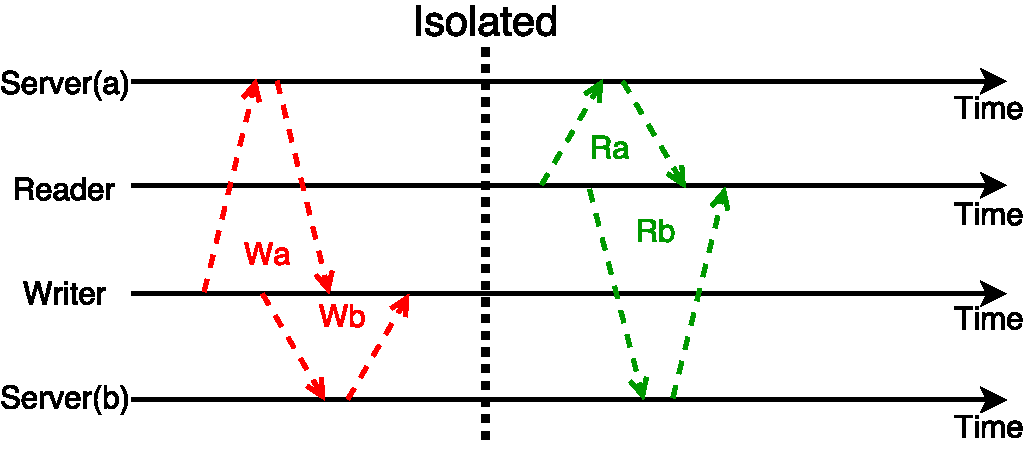
\includegraphics[width=0.48\textwidth]{images/read_write_isolation.pdf}
\caption{Two senders issue read and write requests to two receivers.}
\label{fig:example}
\end{figure}



\begin{figure}[t]
\centering
	\subfloat[Lock-based.\label{fig:concurrency-lock}]
	{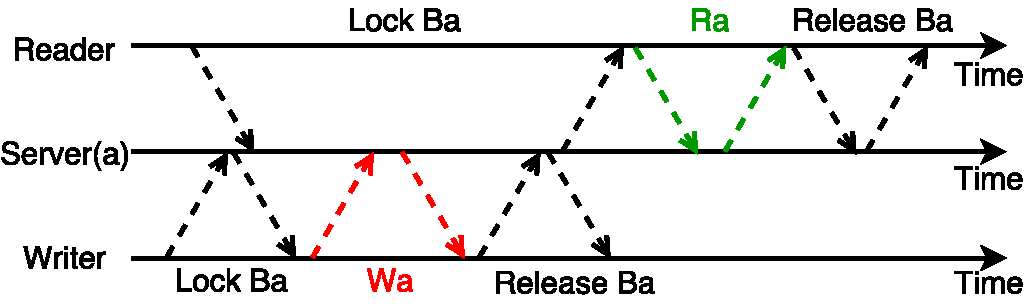
\includegraphics[width=.45\textwidth]{images/LockBased.pdf}}
    \hspace{0in}
	\subfloat[Timestamp-based (OCC).\label{fig:concurrency-timestamp}]
	{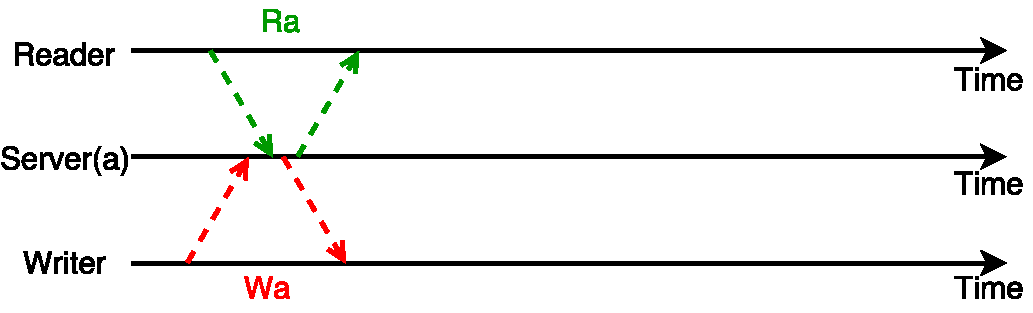
\includegraphics[width=.45\textwidth]{images/TimestampBased.pdf}}
	\caption{Two concurrency control mechanisms for distributed transactions.}
	\label{fig:concurrency-control}
\end{figure}
\fi



%The story begins with a hypothetical distributed banking system. Two accounts Alice and Bob are stored in different \textit{shards} at distant locations. Initially, their balances are $B_a$ and $B_b$. When Alice transfers \$1 to Bob, two write operations are sent to the shards: $B_a -= 1$ and $B_b += 1$, call them $W_a$ and $W_b$. At the same time, an auditor checks the total balance in the bank by accumulating balances of all accounts, resulting in two read operations: $R_a$ and $R_b$.
%If the system does not support transactions, the ordering of events may be $W_a < R_a < R_b < W_b$, then the auditor would find an inconsistent total balance.

%It is worth noting that \sys ensures ordering instead of consensus. When some hosts experience failure, \sys does not ensure a quorum of hosts agree on its received messages. NOPaxos~\cite{li2016just} has shown that \sys leads to an efficient implementation of distributed consensus.

%\subsection{Reliable Ordered Message Scattering}

%We propose reliable ordered message scattering (\sys), which ensures a group of messages to be scattered atomically and obey causality and total order.
%A \textit{message scattering} $S$ is a group of $n$ (potentially different) messages $M_1^s, \ldots, M_n^s$ sent from a sender host $H^s$ to $n$ receiving hosts $R_1^s, \ldots, R_n^s$ respectively. A host in the system may send message scatterings to any group of hosts.
%Each host can be both sender and receiver, but we split each host to a sender and a receiver for clarity.
%\sys offers the following properties:~\cite{kshemkalyani2011distributed}

%\parab{Validity.} If the sender $H^s$ and all receivers $R_i^s$ of a message scattering $S$ have no failure, and the network has no permanent failure, each message $M_i^s$ is eventually delivered to $R_i$. No message is delivered more than once.

%\parab{Atomicity.} The set of messages $M_i^s$ in a message scattering $S$ are either all got delivered or none got delivered.

%\parab{Total Order.}The message scatterings are total ordered. For any pair of message scatterings $S_1$ and $S_2$, if a message in $S_1$ is delivered before $S_2$ to a receiver, then message in $S_1$ are delivered before $S_2$ to any other receiver that receives messages from both scatterings. 

%\parab{FIFO.}For each pair of message scatterings $S_1$ and $S_2$ with a same sender $H$ and share a same receiver $R$, $S_1$ is delivered before $S_2$ at $R$ if and only if $S_1$ is sent before $S_2$ by $H$.

%\parab{Causality.}The total order of message scatterings preserves causality. For a pair of scatterings $S_1$ and $S_2$, if the sender of $S_1$ is a receiver of $S_2$, and $S_2$ is sent after receiving $M \in S_1$, then $S_1$ is ordered before $S_2$.

%\sys can remove all three hazards in Sec.\ref{subsec:tso}.

%We implement the total order of message scatterings using explicit timestamps.
%Each sender assigns a monotonically increasing timestamp to each message scattering.
%Each receiver delivers messages according to timestamp order (break ties by sender ID).

\iffalse
\subsection{Use Cases}
\label{subsec:application-scenarios}

In this section, we discuss three use cases of \sys.
These cases are used to illustrate how \sys can help simplify distributed systems construction, and they are by no means the only usage scenarios where \sys can be useful.
%By avoiding IRIW hazard, independent distributed transactions can complete in one round-trip with high throughput under contention.
%By avoiding IMW hazard, log replication can be both scalable and serializable, which is a building block for both strongly and eventually consistent replicated systems.
%By avoiding WAW hazard, \sys improves consistency in distributed shared memory.

\subsubsection{Distributed Independent Transactions}
\label{subsec:transactional-kvs}
We consider \emph{independent transactions} or \emph{one-shot transactions}~\cite{kallman2008h}, in which the transaction involves multiple shards but the input of each shard does not depend on output of other shards.
For example, YCSB+T workload for transactional key-value store~\cite{dey2014ycsbt} and the two most frequent transactions in TPC-C benchmark (New-Order and Payment)~\cite{tpcc} are independent transactions.
General transactions can be divided into independent transactions exactly as in Eris~\cite{eris}.
In \sys, we implement each independent transaction as a message scattering to multiple sites.
Transaction initiator uses the scattering timestamp as the transaction timestamp.
\sys guarantees atomicity and isolation, thus solving the concurrency control problem.
Transactions would not abort due to out-of-order operations.
Because \sys assigns timestamps on senders, there is also no sequencer bottleneck.
In this way, independent transactions can complete in a single round-trip, close to a non-transactional system.% (if not counting replication and logging).

%Concurrency control mechanisms of distributed transactions typically fall in two categories~\cite{bernstein1981concurrency}.
%One category uses \textit{locks} to protect accesses to shared resources.
%In this way, the transaction throughput is bounded by the RTT between clients and storage sites.
%The other category is \textit{timestamp ordering}, which assigns a \textit{timestamp} to each transaction, and transactions are serialized according to timestamp order~\cite{kung1981optimistic,bernstein1983multiversion}.
%Due to variable network delay and multiple paths in the network, sites may receive transactions out-of-order.
%Out-of-order transactions are aborted and retried with a higher timestamp.
%The abort rate increases with the number of concurrent conflicting transactions, and the effective throughput does not scale~\cite{yu2014staring}.
%In addition, timestamp assignment often requires a centralized sequencer, which limits scalability~\cite{yu2014staring}.

%We follow the timestamp ordering approach.
%First, we consider one-shot transactions~\cite{kallman2008h} or single round-trip transactions, in which the transaction involves multiple sites but the input of each site does not depend on output of other sites.
%For example, YCSB+T workload for transactional key-value store~\cite{dey2014ycsbt} and the two most frequent transactions in TPC-C benchmark (New-Order and Payment)~\cite{tpcc} are one-shot transactions.
%In \sys, we implement each transaction as a message scattering to multiple sites.
%Transaction initiator uses the scattering timestamp as the transaction timestamp.
%\sys guarantees atomicity and isolation, thus solving the concurrency control problem.
%Transactions would not abort due to out-of-order operations.
%Because \sys assigns timestamps on senders, there is also no sequencer bottleneck.
%In this way, one-shot transactions can complete in a single network RTT (if not counting replication and logging).
%
%Second, we consider general transactions in which the read set and write set is known at the beginning of transaction.
%In \sys, each transaction scatters its read and write sets to the involved sites when transaction begins.
%Each site builds a dependency graph of read and write operations, and executes transactions according to it.
%During transaction execution, messages do not need to go through \sys.
%Because each site receives read and write sets in transaction timestamp order, writes would not be reordered with previous reads during transaction execution, thus eliminating transaction aborts caused by write conflicts.


\iffalse
Memory consistency and log replication motivate the need of total order multicast, where one message is sent to multiple receivers.
In addition, applications need serializable execution of a group of operations~\cite{cheriton1994understanding}, \textit{e.g.} accessing metadata and data.
If a group of operations involves multiple nodes in a distributed system, the communication pattern is \textit{message scattering}, where one sender scatters potentially different messages to multiple receivers.
The messages in a scattering should be ordered \textit{atomically}, such that a) either all or none receivers deliver the messages, b) all messages are delivered at the same serialization time.
The IMW and IRIW cases in Sec.\ref{subsec:tso} are examples of \RED{atomic message scattering or just message scattering?} message scattering.
In IMW, access and error log of a request compose a scattering.
In IRIW, two read requests and two write requests each compose a scattering.

Atomic message scattering can solve the concurrency control problem of one-shot transactions~\cite{kallman2008h} (or called single round-trip transactions), in which the transaction involves multiple sites but the input of each site does not depend on output of other sites.
For example, the two most frequent transactions in TPC-C benchmark (New-Order and Payment)~\cite{tpcc} are one-shot transactions.

\RED{is here sounds like 'there are only two categories?'} There are two categories of concurrency control~\cite{bernstein1981concurrency}.
One category uses \textit{locks} to protect accesses to shared resources.
In this way, the transaction throughput is bounded by the RTT between the clients and the shards.
The other category is \textit{timestamp ordering}, which assigns a \textit{timestamp} to each transaction, and transactions are serialized according to timestamp order~\cite{kung1981optimistic,bernstein1983multiversion}.
Due to variable network delay \RED{and multi-path?}, shards may receive transactions out-of-order.
Out-of-order transactions are aborted and retried with a higher timestamp.
The abort rate increases with the number of concurrent conflicting transactions, and the effective throughput does not scale~\cite{yu2014staring}.
In addition, timestamp assignment often requires a centralized sequencer, which limits scalability~\cite{yu2014staring}.

We implement an one-shot transaction as a total-order message scattering, which ensures that shards process transactions in timestamp order, therefore eliminating transaction aborts and centralized timestamp assignment.
\RED{doesn't make sense, ensure process in timestamp order has nothing to do with centralized timestamp assignment. may be: 'which requires no centralized timestamp assignment and ensures that shards process transactions in timestamp order without out-of-order aborts.' is better}
\fi

%In the absence of packet loss and node failure, total-order scattering can complete in an RTT, adding little latency and bandwidth overhead compared to traditional message scattering.

%We will use a hypothetical banking example to illustrate the main concepts. Two accounts Alice and Bob are stored in different \textit{shards} at distant locations. Initially, their balances are $B_a$ and $B_b$. When Alice transfers \$1 to Bob, two write operations are sent to the shards: $B_a -= 1$ and $B_b += 1$, call them $W_a$ and $W_b$. At the same time, an auditor checks the total balance in the bank by accumulating balances of all accounts, resulting in two read operations: $R_a$ and $R_b$. If the system does not support transactions, the ordering of events may be $W_a < R_a < R_b < W_b$, then the auditor would find an inconsistent total balance.

%A strongly consistent distributed system requires the reads and writes to be \textit{transactional}. The transaction $R_a, R_b$ and the transaction $W_a, W_b$ need to be performed in isolation.

%There are two main categories of concurrency control to implement a transactional system. One category uses \textit{locks} to protect accesses to shared resources. The read transaction needs to lock $B_a$ and $B_b$, and the write transaction also needs to lock them. The transaction throughput is bounded by the \textit{round-trip time} (RTT) between the clients and the shards, because the lock must be sent from the shard to the client, then the client may send unlock to the shard.
%In our example scenario where all transactions need to lock a single resource, if the RTT is 100~$\mu$s, the throughput is bounded to 10K transactions per second.

%The other category is \textit{optimistic concurrency control} (OCC). It assigns a \textit{timestamp} to each transaction ($T_R$ for read, $T_W$ for write) and tracks object accesses during transaction execution. Transactions are serialized according to timestamp order. Once the system detects a \textit{late write}, that is, the write operation has lower timestamp than a read operation ($T_W < T_R$) but arrives later ($R_a < W_a$ or $R_b < W_b$), one of the transactions needs to be aborted and retried with a higher timestamp.
%Due to variable delays between clients and shards, if the read and write transactions are initiated at almost the same time, there are many possible orderings of $R_a, R_b, W_a, W_b$ and $T_R, T_W$. 
%If the network delays between clients and shards follow a normal distribution, for two conflicting concurrent transactions, the probability of aborting one transaction is 3/4 with two shards. If each transaction involves $N$ shards, the abort probability is $1-(\frac{1}{2})^N$.

%If we regard each transaction as an event on a client, then the \textit{event timestamp} is the transaction timestamp. The read and write operations are the effects of the events, which propagate to the shards via messages.
%Each event may \textit{scatter} a set of messages to receivers (shards in our example). Each message is tagged with the event timestamp. Different messages may be scattered to different receivers, so \textit{broadcast} is a special case of \textit{scatter}.

%To implement OCC without transaction aborts, we propose \textit{total-order message scattering} (\sys). \sys assigns timestamps to events and scatters messages from events, so that each host delivers messages to applications in monotonically increasing timestamp order (break ties by sender ID).
%\sys provides a total ordering of all events in a distributed system, and ensures that each node observes the events (via messages) consistent with the total ordering.
%With \sys, we regard each single-round-trip transaction as an event on the transaction initiator. In the absence of failure, transaction abort in OCC will never be triggered, because the read and write operations are always received by shards in the same ordering according to transaction timestamps.


%In the distributed system, multiple \textit{hosts} are connected via the network. %A distributed system is made up of multiple \textit{hosts} connected via network. 
%An \textit{event} occurs on a host, and scatters messages to other hosts. For example, a distributed single-round-trip transaction can be regarded as an event on the transaction initiator, and its read and write operations are sent to the shards where the objects are stored. Here we use the term \textit{scatter} instead of \textit{multicast} because each shard only needs to receive operations related to the objects it host.


%Recent years there is rich literature on improving eventual consistency in geographically replicated systems . The CAP theorem suggests that sequential consistency is not possible if both read and write operations have latency lower than inter-datacenter delay.

%COPS and Eiger provide causal+ consistency in geo-replicated systems by tracking dependency of values or operations at shared storage servers. Causal consistency rules out WAW hazard. To rule out SAW hazard, message passing needs to be taken into account when tracking potential causal dependencies. Although causal+ ensures per-key sequential consistency by serializing the update log of each key, in the IRIW case, the change order observed by C and D may eventually diverge, because A and B are different keys. Furthermore, eventually consistent systems typically do not provide a bounded delay of convergence.

%We build each replica as a transactional key-value store, and deploy another instance of reliable TOMS for replication traffic. TOMS serializes updates from all remote replicas. Applying the last-writer-wins rule on the timestamps of local objects and remote updates, the system will be eventually consistent, without the need of tracking causal dependencies or a convergent conflict handling function. TOMS also provides bounded convergence delay. After receiving replication at timestamp T and resolving conflicts, we are sure that the history before T will never be changed. Furthermore, we no longer need to replicate to all replicas to ensure total ordering of updates (cite The Potential Dangers of Causal Consistency and an Explicit Solution, SOCC'12).

\subsubsection{Serializable Log Replication}
\label{subsec:log-replication}

A canonical application of \sys is \textit{serializable log replication}~\cite{birman1985replication,petersen1997flexible,belaramani2006practi}.
Distributed databases are replicated for reliability and performance.
When multiple replicas process write operations in parallel, the consistency among replicas is a paramount challenge.
%The PACELC theorem~\cite{abadi2012consistency} suggests that even when a system has no failure and network partition, one has to choose between latency (L) and consistency (C).
%On one end of the spectrum are strongly consistent systems~\cite{kallman2008h,li2012making,corbett2013spanner}, where each replica processes read operations locally and waits an RTT for write operations to propagate to all replicas.
%Low latency data center networks enable an increasing number of intra-datacenter databases embrace strong consistency.
%On the other end of spectrum are eventually consistent systems~\cite{terry1995managing,lloyd2011don,lloyd2013stronger}, where both read and write operations are processed locally, and conflicting write operations are merged in a deterministic way.
%Due to high latency among data centers, many geographically replicated databases choose eventual consistency.

%Due to scalability concerns of log serialization~\cite{anna}, there has been extensive work to track dependency and ensure convergent conflict resolution at application level~\cite{lloyd2011don,lloyd2013stronger}.
%First, most of these approaches do not ensure all 
%Second, they cannot say ``for sure'' in the presence of out-of-band communication~\cite{cheriton1994understanding}, \textit{e.g.} cannot avoid SAW hazard if send operation is not tracked in the dependency graph.
%In addition to higher consistency, total order communication provides an explicit time of convergence.
%After receiving replication of timestamp $T$, we are sure that the history before $T$ will never be changed.

By removing IMW hazard, \sys ensures that each replica receives an identical sequence of write operations from all other replicas.
If write operations are blocked until receiving potentially conflicting writes, \textit{i.e.} insert a memory barrier after each write, the system is sequentially consistent because each operation can be serialized at its beginning time~\cite{lu2016snow}.
If write operations are returned immediately while changes propagate, because local read operations may occur during propagation, the system is not sequentially consistent, but causality is preserved~\cite{terry1995managing}.
Further, applying the Thomas write rule~\cite{thomas1979majority} on the timestamps of local and remote updates achieves eventual consistency.
%The reasoning above assumes reads are local and writes are propagated.
%Similar reasoning applies to write-intensive systems where writes are local, while each read operation retrieves from multiple replicas and return the latest version.
%\sys also ensures sequential consistency in this case.

\subsubsection{Total Store Ordering in DSM}

Recent x86 processors provides a \textit{total store ordering} (TSO) memory model~\cite{sewell2010x86} in which each core observes a consistent ordering of writes from all other cores, thus being causally and eventually consistent.
TSO reduces synchronization in concurrent programming~\cite{morrison2013fast,tassarotti2015verifying}.
Obviously, a distributed shared memory (DSM) system built upon \sys achieves TSO.

In addition, \sys enables an efficient and scalable implementation of \textit{memory barrier}.
The caller blocks itself and sends a null message to itself via \sys with timestamp $T$. Then it unblocks upon receiving the message at time $T'$.
The causality property of \sys ensures that all messages sent before $T$ are received at $T'$.

\iffalse
\textcolor{red}{I think the following paragraph is useless.}
\RED{gefei: yes, I think any explanation can be removed. marked in red}
%These ordering anomalies have been studied extensively in shared memory systems~\cite{gharachorloo1990memory}.
%Recent processors provide higher memory consistency models.
 \RED{where each core observes a consistent ordering of writes from all other cores}.
\RED{In other words, remote writes are propagated via total order communication.}
TSO eliminates SAW and WAW ordering anomalies above and reduces synchronization in concurrent programming~\cite{morrison2013fast,tassarotti2015verifying}.
\RED{In addition, TSO makes \textit{memory barrier} easy to implement without locking the bus.
The barrier initiator core blocks itself and sends a message to itself via total order communication, and unblocks upon receiving the message.}
In this paper, we extend the concept of TSO to distributed systems, providing same consistency as multi-core processors.
In Sec.\ref{subsec:transactional-kvs}, we introduce a novel message scattering primitive to remove IMW and IRIW hazards.
%Concretely, each message is assigned a monotonically increasing timestamp at the sender and each receiver processes messages in timestamp order (break ties by sender ID).
\fi






\subsection{Existing Approaches}
\label{subsec:existing-approaches}

Since the dawn of distributed system research~\cite{lamport1978time}, there has been extensive research in ordered communication, mostly providing a multicast or broadcast primitive.
To achieve linearizable ordering, one line of work leverages logically centralized coordination, \textit{e.g.}, centralized sequencers~\cite{eris} or a token passed among senders or receivers~\cite{rajagopalan1989token,kim1997total,ekwall2004token}.
As a result, it is challenging to scale the system.
Another line of work uses fully distributed coordination, \textit{e.g.}, exchange timestamps among receivers before they start to process messages~\cite{lamport1978time}, or aggregate history during message delivery~\cite{chandra1996unreliable}.
This causes extra network communication overhead and delay, thus degrading system efficiency.
A third line of work assumes a synchronous network, \textit{e.g.}, the block generation interval in Bitcoin blockchain~\cite{nakamoto2008bitcoin} is designed to be higher than the maximum delay among hosts.
However, in data center systems, waiting for worst-case delay leads to unacceptable latency.

To achieve reliability in the presence of failures, we need to achieve consensus among receivers.
Most existing works, e.g. Paxos~\cite{lamport1998part} and Zab~\cite{junqueira2011zab}, use voting to guarantee that a quorum of receivers agree on the sequence of messages to be delivered.
The votes need to be broadcast to and collected from all hosts, incurring significant communication overhead for hundreds of thousands of hosts in a data center.
In addition, Paxos does not allow Byzantine failure of hosts, which is insecure for a multi-tenant data center service with potentially malicious hosts.
Achieving Byzantine fault tolerance~\cite{lamport1982byzantine,castro1999practical,kotla2007zyzzyva} in an asynchronous network is notably complicated and inefficient~\cite{mickens2014saddest}.

Critics and proponents of causal and totally ordered communication (CATOCS) have long discussed the pros and cons of such a primitive~\cite{cheriton1994understanding,birman1994response,van1994bother}. 
\sys achieves scalability with in-network computation and incurs little overhead, thus removing one of the biggest criticisms of this primitive.

Recent years witness a trend of co-designing distributed systems with programmable network switches.
Mostly Ordered Multicast~\cite{ports2015designing} and NOPaxos~\cite{li2016just} use a switch as a centralized sequencer or serialization point to achieve fast consensus.
However, consensus does not imply FIFO ordering~\cite{junqueira2011zab}.
Eris~\cite{eris} proposes in-network concurrency control using switch as a centralized sequencer.
%To mitigate the single point of failure, NetChain~\cite{jin2018netchain} uses a chain of switches for fault tolerance.
Each transaction in Eris must go through the centralized sequencer and involve all shards and replicas.
However, in large distributed services, most transactions only involve a small portion of shards~\cite{nishtala2013scaling}, so sending null messages to other shards incurs high overhead.
In addition, when all hosts are correct, an Eris transaction may fail due to packet loss, while subsequent transactions from the same sender may succeed, violating validity of \sys.
Further, none of these works tolerate Byzantine host failure.
\sys follows the trend of systems and network co-design to achieve scalability, efficiency and security.

\fi

%It works like a merge sort: Each step the network switch compares the heads of input streams and output the head packet with minimum timestamp. %Reordering packets on the switch introduces less reordering delay compared to reordering on the receivers (as shown in Figure~\ref{fig:barrier}), because the switch sees messages more frequently~\cite{aguilera2000efficient}.
%However, when the timestamps are not perfectly synchronized, the switch needs to wait and buffer other streams.
%The maximum time of waiting equals the network delay variance plus the clock skew among senders. According to Sec.\ref{sec:goals}, the delay variance may be milliseconds, therefore for a 40~Gbps network, the switch needs a 5~MB buffer per port to hold out-of-order packets.

%The predominant approach to total order communication is consensus protocols~\cite{lamport1998part,raft}, which introduces a centralized serialization point (not necessarily on the data path, but at least requires a centralized sequencer~\cite{kaminsky2016design}).

%they cannot say ``for sure'' in the presence of out-of-band communication~\cite{cheriton1994understanding}

\iffalse
\subsection{Design Goals}
\label{sec:goals}

Our goal is to build a ordered message scattering service that satisfies the following requirements.

%\textbf{Correctness.}
%A sender scatters a group of messages with a same timestamp to multiple receivers, called a \textit{scattering}.
%Timestamps for different scatterings are unique and increasing on each sender.
%Each receiver delivers messages to applications in timestamp order (break ties by sender ID).
%Messages in each scattering are delivered by either all or none receivers.

\parab{Efficient.}First, the \textit{reordering delay} between end host receiving the message and delivering the message to application should be minimal.
This requires senders to assign timestamps properly so that messages with similar timestamps arrive at receivers as synchronized as possible.
Second, the network and computation overhead of the system should be minimal.

\parab{Scalable.}The system should be scalable with number of switches and hosts, which implies no central coordinator and the overhead should not increase too much as the system scales out.
%Additionally, for ease of deployment, it is also desirable for the algorithms running on each host and switch to be logically equivalent.



%\textbf{Low Network Bandwidth Overhead.}
%Additional packets generated for ensuring ordering should be minimal. The metadata tagged on each packet should also be minimal.

%\textbf{Low CPU Overhead.}
%Because the CPUs on switches are typically not very powerful, the processing on switch CPU should be as simple and infrequent as possible. Moreover, the reordering overhead on end hosts should also be reasonable.

\parab{Fault Tolerant.}The correctness of the system should not be violated under packet loss, or failure of switches, links or end hosts.
The system ensures liveness unless network partition occurs.


\parab{Readily Deployable.}The service should be readily deployable using commodity data center switches.

%\textbf{Adaptive to Delay Variance.}
%The delay among geographically distributed datacenters can be hundreds of milliseconds.
%Because commodity NIC hardware is not able to assign a same timestamp to a group of scattered messages, \sys assigns timestamps in software.
%Different OS network stacks have more than 100~$\mu$s of processing delay differences, and it may grow to milliseconds under heavy load.
%Links with different speeds or congestions also lead to delay variations.
%The system should dynamically adapt to the variance of network delays to minimize reordering delay.
\fi
